
\section{Carrier-Greenspan periodic solution}

Periodic solutions for flows on a sloping beach were proposed by Carrier and Greenspan~\cite{CG1958}. The solutions have been widely used to test the performance of numerical methods used to solve the shallow water equations~\cite{Johns1982,MR2012CG}.

This test can be described in dimensional and dimensionless equations. For our reference, please note that dimensional quantities shall be denoted by starred variables, while dimensionless quantities by unstarred variables for brevity of our analytical presentation. This notational convention is used only in this test.

The problem is set up as follows. Consider a one dimensional domain through the $x^*$-axis. Recall the shallow water equations
\begin{equation} \label{eq:mass_app}
h^*_{t^*} +\left(h^*u^*\right)_{x^*}=0\,,
\end{equation}
\begin{equation} \label{eq:mom_app}
\left(h^*u^*\right)_{t^*}+\left(h^*{u^*}^2+\frac{1}{2}g{h^*}^2\right)_{x^*}=-gh^* z^*_{x^*}\,.
\end{equation}
Here,
$x^*$ represents the one-dimensional domain,
$t^*$ is the time variable,
$u^*=u^*(x^*,t^*)$ represents the velocity,
$z^*=z^*(x^*)$ denotes the water bed topography (elevation),
$h^*=h^*(x^*,t^*)$ denotes the height (water depth), that is, the distance from the free surface to the water bed topography, and
$g$ is the acceleration due to gravity.
Now, consider the situation on a sloping beach. The topography changes linearly with $x^*$
\begin{equation}
z^*=(h_0^*/L^*)x^*-h_0^*\,,
\end{equation}
in which $h_0^*$ is the vertical distance from the origin $O$ to the topography at any time, and $L^*$ is the horizontal distance from the origin $O$ to the topography when the water is still. This implies that when the water is still: $z^*=-h^*$ over the spatial domain, $z^*=-h_0^*$ at $x^*=0$\,, and the position of the shoreline is $x^*=L^*$\,. More detailed descriptions are given by Mungkasi and Roberts~\cite{MR2012CG}.



The free surface or called stage is defined by $w^*:=h^*+z^*$\,.
Scaling the horizontal distance by $L^*$\,, the vertical distance by $h_0^*$\,, the time by $L^*/\sqrt{gh_0^*}$\,, and the velocity by $\sqrt{gh_0^*}$\,, the nonconservative dimensionless shallow water equations can be expressed as
\begin{equation} \label{eq:mass1_app}
w_t + \left[ \left( w+1-x  \right)u  \right]_{x} = 0\,,
\end{equation}
\begin{equation} \label{eq:mom1_app}
u_t + u u_x + w_{x} = 0\,.
\end{equation}
For smooth solutions, equations (\ref{eq:mass1_app}) and (\ref{eq:mom1_app}) are equivalent to the conservative dimensionless shallow water wave equations
\begin{equation}
h_t + \left( hu \right)_x = 0\,,
\end{equation}
\begin{equation}
\left(hu\right)_t + \left( hu^2 + \frac12 h^2  \right)_x = -h z_x\,.
\end{equation}


Carrier and Greenspan showed that
\begin{equation} \label{eq:w_johns_full}
w = - \frac12 u^2 + \mathcal{A} J_0 \left( \frac{4 \pi \sqrt{ w+1-x}}{T} \right) 
\cos{\left(\frac{2 \pi \left( u+t \right)}{T}\right)}\,,
\end{equation}
\begin{equation} \label{eq:u_johns_full}
u = - \frac{\mathcal{A}J_1\left( \frac{4 \pi \sqrt{w+1-x}}{T}  \right)}{\sqrt{w+1-x}}
 \sin{\left( \frac{2 \pi \left(u+t \right)}{T}  \right)}\,
\end{equation}
satisfies the shallow water equations. This was verified by Johns~\cite{Johns1982} as well as Mungkasi and Roberts~\cite{MR2012CG}. Equations (\ref{eq:w_johns_full}) and (\ref{eq:u_johns_full}) are the Carrier--Greenspan periodic solutions for flows on a sloping beach, which are written in the dimensionless form. Obviously, this can be rescalled back to the dimensional form.


Because this solution is periodic, the initial condition can be set by substituting $t=0$ into the analytical solution (\ref{eq:w_johns_full}) and (\ref{eq:u_johns_full}).


\subsection{Results}

We consider a spatial domain given by the interval $[-50, 55050]$\,. The dimensional length is $L^*=50,000$\,, dimensional height $h_0^*=500$\,, and dimensional period $T^*=900$\,. At $x^*=0$ the dimensional amplitude is $\epsilon^*=1.0$\,. After four cycles, periodic motions are clear.

The following figures show the stage, $x$-momentum, and $x$-velocity at several instants of time through a cross-section of the domain. Perturbation at the zero point of the spatial domain is also shown.
We should see excellent agreement between the analytical and numerical solutions.

\begin{figure}
\begin{center}
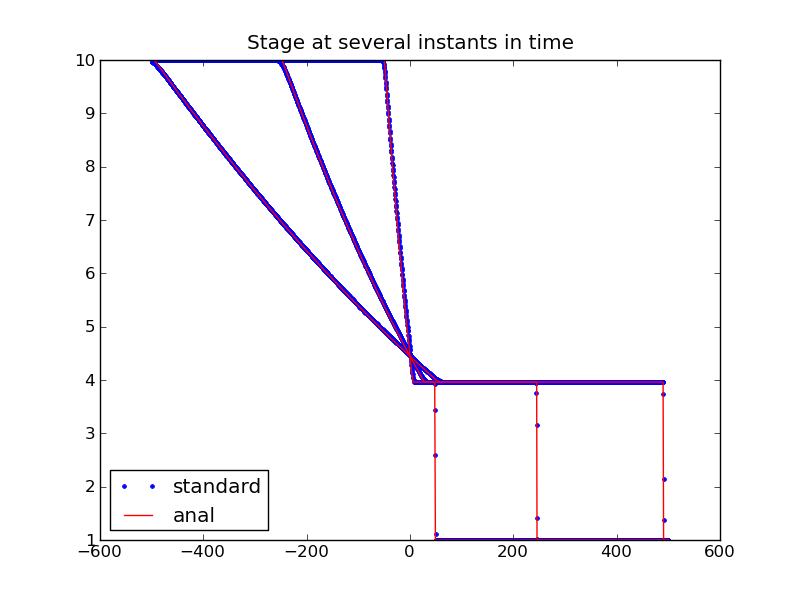
\includegraphics[width=0.9\textwidth]{stage_plot.png}
\end{center}
\caption{Stage results}
\end{figure}

\begin{figure}
\begin{center}
\includegraphics[width=0.9\textwidth]{xmom_plot.png}
\end{center}
\caption{Xmomentum results}
\end{figure}

\begin{figure}
\begin{center}
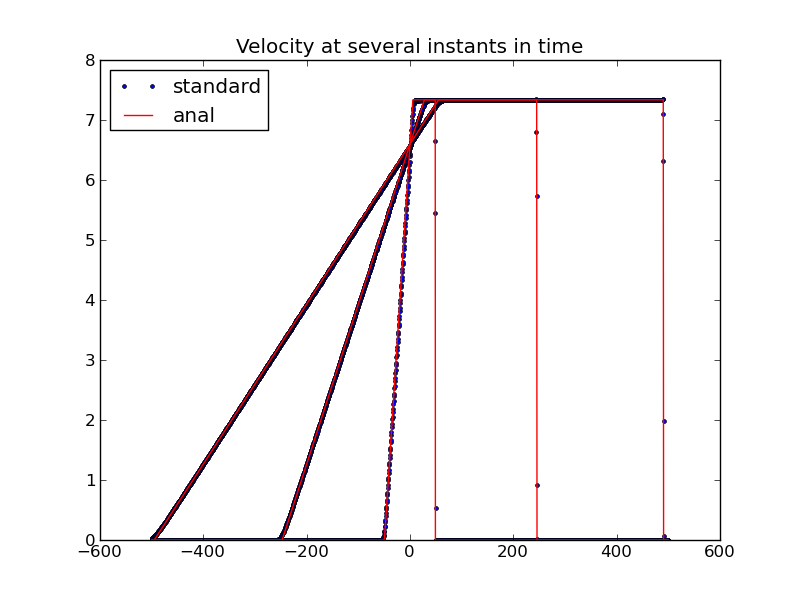
\includegraphics[width=0.9\textwidth]{xvel_plot.png}
\end{center}
\caption{Xvelocity results}
\end{figure}


\begin{figure}
\begin{center}
\includegraphics[width=0.9\textwidth]{perturbation_at_origin.png}
\end{center}
\caption{Velocity results}
\end{figure}


\endinput
